\chapter{Creating networks} \label{ch:creation}

Networks can be created in multiple ways: manually, that is, individually adding vertices and edges as seen above, or calling functions which create standard types of graphs, or using input/output functions, or using network generation models. All these (apart from manual creation) are reviewed in this chapter.

\section{Standard graphs}

The following pre-defined graphs can be created. The corresponding networks are shown in Figure \ref{fig:notable}.
\begin{lstlisting}[style=c++] 
#include "generation/standard_graphs.hpp"
auto n_5 = null_graph(5);
auto p_5 = path_graph(5);
auto c_5 = cycle_graph(5);
auto w_5 = wheel_graph(5);
auto k_5 = complete_graph(5);
auto k_3_2 = complete_bipartite_graph(3, 2);
\end{lstlisting}

\begin{figure}
  \centering
\begin{subfigure}{.26\textwidth}
  \centering
  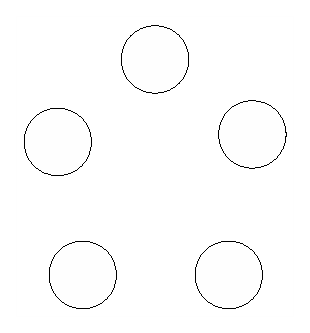
\includegraphics[width=.8\linewidth]{figs/N5.eps}
  \caption{$N_5$}
  \label{fig:notable-N5}
\end{subfigure}
\begin{subfigure}{.26\textwidth}
  \centering
  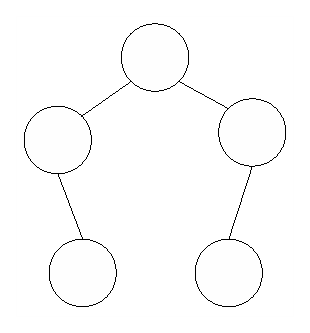
\includegraphics[width=.8\linewidth]{figs/P5.eps}
  \caption{$P_5$}
  \label{fig:notable-P5}
\end{subfigure}
\begin{subfigure}{.26\textwidth}
  \centering
  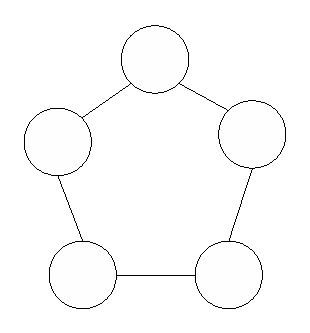
\includegraphics[width=.8\linewidth]{figs/C5.eps}
  \caption{$C_5$}
  \label{fig:notable-C5}
\end{subfigure}
\newline
  \centering
\begin{subfigure}{.26\textwidth}
  \centering
  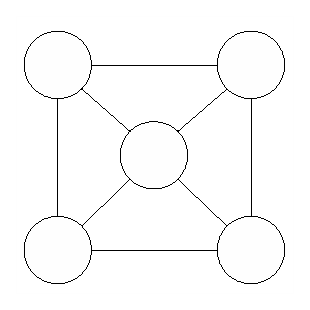
\includegraphics[width=.8\linewidth]{figs/W5.eps}
  \caption{$W_5$}
  \label{fig:notable-W5}
\end{subfigure}
\begin{subfigure}{.26\textwidth}
  \centering
  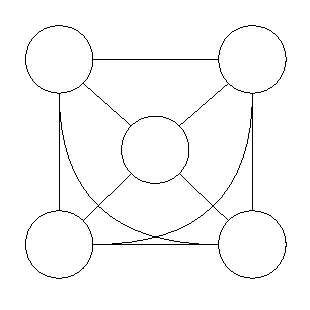
\includegraphics[width=.8\linewidth]{figs/K5.eps}
  \caption{$K_5$}
  \label{fig:notable-K5}
\end{subfigure}
\begin{subfigure}{.26\textwidth}
  \centering
  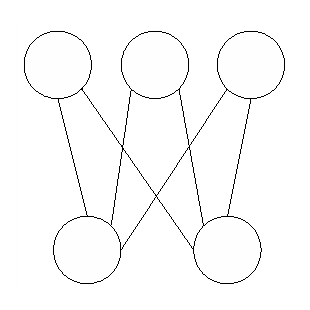
\includegraphics[width=.8\linewidth]{figs/K23.eps}
  \caption{$K_{2,3}$}
  \label{fig:notable-K23}
\end{subfigure}
\caption{Special graphs: null graph, path graph, cycle graph, wheel graph, complete graph, complete bipartite graph}
\label{fig:notable}
\end{figure}



\section{I/O}  \label{ch:io}

The general syntax to read a network from file is the following:

\begin{lstlisting}[style=file]
#VERSION           
2.0                
                   
#TYPE              
directed           
                   
#VERTEX ATTRIBUTES 
a1,string          
                   
#EDGE ATTRIBUTES   
a1,double          
                   
#VERTICES          
v1,a_value         
v2,another_value   
v4,one_more_value  
                   
#EDGES             
v1,v2,2.3          
v1,v3,4            
v2,v1,3            
v1,v4,4.2          
\end{lstlisting}
By default edges are undirected, so if no attributes are present the following is also a valid input file:
\begin{lstlisting}[style=file]
v1,v2              
v1,v3              
v1,v4              
\end{lstlisting}
Under \#TYPE we can also specify whether the network is weighted:
\begin{lstlisting}[style=file]  
#TYPE              
directed           
weighted    
\end{lstlisting}        
If the network is weighted, then the first attribute value for edges must be the weight:
\begin{lstlisting}[style=file]         
#EDGES             
v1,v2,143,2.3      
v1,v3,11,4         
v2,v1,14,3         
v1,v4,10,4.2       
\end{lstlisting}
    
Multilayer networks allow to specify the features of each layer, and also differentiate between actors and vertices:
\begin{lstlisting}[style=file]
#TYPE                
multilayer           
                     
#VERSION             
2.0                  
                     
#LAYERS              
l1,l1,UNDIRECTED     
l2,l2,UNDIRECTED,LOOPS
l1,l2,DIRECTED       
                     
#ACTOR ATTRIBUTES    
ssn, string          
                     
#ACTORS              
v1,122343242         
v3,122343654         
                     
#VERTEX ATTRIBUTES   
l2,day,string        
                     
#VERTICES            
v6,l2,Monday         
                     
#EDGE ATTRIBUTES     
l1,attr1,numeric 
attr2,numeric   
                     
#EDGES               
v1,l1,v2,l1,1,7      
v1,l1,v5,l1,2,8      
v2,l1,v5,l1,3,9      
v2,l1,v3,l1,4,10     
v2,l1,v4,l1,5,11     
v3,l1,v4,l1,6,12     
v1,l1,v4,l2,13       
v2,l1,v3,l2,14       
v2,l1,v4,l2,15       
v3,l1,v3,l2,16       
v3,l1,v4,l2,17       
v1,l1,v2,l2,18       
\end{lstlisting}
In the example above, attr1 is an attribute of edges in layer 1, while attr2 is a global attribute.


Edges in a multiplex network are instead expressed only specifying the layer once, as interlayer edges are not allowed:

\begin{lstlisting}[style=file]              
l1,v1,v2,1,7      
l1,v1,v5,2,8  
\end{lstlisting}

\emph{Note: after the introduction of cubes we may define a new input format that allows more flexibility, without breaking backward compatibility. Working on it.}

\section{Generation}  \label{ch:generation}

Three types of network generation approaches are currently available. ER models for simple graphs, multilayer network co-evolution, and multilayer community-based.

\subsection{Simple graphs}

ER graphs can be created using either the np model, specifying the number of vertices and the probability for every pair of vertices of being adjacent, or the nm model, specifying the number of vertices and the number of edges:
\begin{lstlisting}[style=c++]
auto er_np = erdos_renyi_np(10, .2);
auto er_nm = erdos_renyi_nm(10, 4); 
\end{lstlisting}

\subsection{Multilayer network coevolution}

Multilayer networks can be generated using a co-evolutionary model where, for every layer, we specify the probability that the layer evolves according to internal dynamics or importing an edge from another layer. A dependency matrix is used to specify from which other layers the edge can be imported, and with which probability.
\begin{lstlisting}[style=c++]
vector<string> layer_names = {"l1", "l2"};
vector<double> pr_internal_event = {.8, .5};
vector<double> pr_external_event = {0, .5};
vector<vector<double>> dependency = {{0, 1}, {1, 0}};
\end{lstlisting}
The internal evolution dynamic is specified in the form of an evolution model, either connecting vertices uniformly at random (\code{ERModel}) or using preferential attachment (\code{PAModel}).
\begin{lstlisting}[style=c++]
vector<EvolutionModel<MultilayerNetwork>*> ev_model;
auto pa = make_unique<PAModel<MultilayerNetwork>>(3, 2);
auto er = make_unique<ERModel<MultilayerNetwork>>(50);
ev_model.push_back(pa.get());
ev_model.push_back(er.get());
\end{lstlisting}
Finally, we have to specify how many evolution steps we want to run:
\begin{lstlisting}[style=c++]
size_t num_of_steps = 100;
\end{lstlisting}
    
The function \code{evolve} takes all these parameters and lets the multilayer network grow. Assume that \code{ml} is a pointer to a multilayer network with two layers.
\begin{lstlisting}[style=c++]
evolve(ml, layer_names,
       pr_internal_event, pr_external_event, 
       dependency, ev_model,
       num_of_steps);
\end{lstlisting}

\subsection{Community-based}

The last way to obtain a multilayer network is by passing a pointer to a community structure as input (see Chapter \ref{ch:community}) specifying the the probability for two vertices of being adjacent if they are inside the same community or in different communities, for each layer. 
\begin{lstlisting}[style=c++]
sample(ml, com, {.5, .5}, {.01, .01});
\end{lstlisting}